\documentclass[10pt,aspectratio=169]{beamer}
\usetheme{metropolis}
\usepackage{booktabs}
\usepackage{tikz}
\usetikzlibrary{positioning,arrows.meta,shapes,fit,backgrounds,calc,patterns}
\usepackage{amsmath,amssymb}
\usepackage{xcolor}

% Fallback if metropolis is not installed: comment out the line above and uncomment:
% \usetheme{default}\usecolortheme{seahorse}

\definecolor{accent}{HTML}{0066CC}
\definecolor{accent2}{HTML}{CC3300}
\definecolor{accent3}{HTML}{009933}
\definecolor{lightgray}{HTML}{F0F0F0}

\title{Cache Optimization with Neural Predictors}
\subtitle{Paper Analysis, Upper-Bound Methodology, and a Bypass-First Plan}
\author{[Your Name]}
\institute{Advisor: [Boss Name]}
\date{Wednesday Briefing}

\begin{document}

% =========================================================
\begin{frame}
  \titlepage
\end{frame}

% =========================================================
\begin{frame}{Research Question}
  \textbf{On which workload classes does which cache policy / predictor help,
  by how much, and at what hardware cost?}

  \vspace{1em}
  Broken into three sub-questions:
  \begin{enumerate}
    \item What does the literature say about \textbf{neural predictors} for caches?
          (accuracy, latency, hardware cost)
    \item What are the \textbf{upper bounds} on each workload class?
          (how much room is even there?)
    \item What is a \textbf{realistic deployable mechanism}?
          (the bypass-first proposal)
  \end{enumerate}

  \vspace{1em}
  \footnotesize\color{gray}
  Framing inherits the Ayers/Litz/Ranganathan 2020 methodology
  (``Classifying Memory Access Patterns''): characterize first, design second.
\end{frame}

% =========================================================
\begin{frame}{Workload Categorization}
  Five access-pattern classes from the Ayers~2020 taxonomy:
  \vspace{0.3em}

  \begin{center}
  \scriptsize
  \begin{tabular}{lp{3.2cm}p{4.8cm}p{2.6cm}}
    \toprule
    \textbf{Class}        & \textbf{Behavior}                   & \textbf{Trace I will use (DPC-3)}                  & \textbf{Availability} \\
    \midrule
    Streaming             & linear scans, low reuse             & \texttt{619.lbm\_s-4268B}                          & \textcolor{accent3}{in DPC-3} \\
    Pointer chase         & dependent loads, irregular          & \texttt{605.mcf\_s-994B}                           & \textcolor{accent3}{in DPC-3} \\
    Indirect              & array-of-pointer, $A[B[i]]$         & \texttt{620.omnetpp\_s-874B}                       & \textcolor{accent3}{in DPC-3} \\
    Branch/control        & control-dependent loads             & \texttt{602.gcc\_s-734B}                           & \textcolor{accent3}{in DPC-3} \\
    Sparse C++            & graph-like XML processing           & \texttt{623.xalancbmk\_s-700B}                     & \textcolor{accent3}{in DPC-3} \\
    \midrule
    Graph (target)        & BFS / PR / SSSP                     & GAP-bench (\texttt{bfs}, \texttt{pr})              & \textcolor{accent2}{NOT in DPC-3} \\
    Server / instr-heavy  & SPECjbb, web workloads              & CloudSuite                                          & \textcolor{accent2}{NOT in DPC-3} \\
    libquantum / mcf 2006 & older streaming / graph             & SPEC2006                                            & \textcolor{accent2}{DPC-3 is 2017} \\
    \bottomrule
  \end{tabular}
  \end{center}

  \vspace{0.5em}
  \footnotesize
  \textbf{If a target trace is missing:}
  GAP / CloudSuite are \emph{not} packaged in DPC-3.
  Substitution plan: \texttt{605.mcf\_s} (memory-intensive graph-like behavior)
  proxies for graph workloads; \texttt{600.perlbench\_s} or
  \texttt{602.gcc\_s} proxies for instruction-heavy workloads.
  Generating GAP traces requires running Intel Pin --- a Week-2+ task,
  not blocking this deck.

  \vspace{0.3em}
  \footnotesize\color{gray}
  Trace list verified at \texttt{dpc3.compas.cs.stonybrook.edu/champsim-traces/speccpu/}.
\end{frame}

% =========================================================
\begin{frame}{Paper Analysis: Neural Predictor Families (1/2)}
  \textbf{Accuracy vs. hardware cost, from each paper's reported numbers:}
  \vspace{0.5em}

  \begin{center}
  \scriptsize
  \begin{tabular}{p{2.4cm}p{2cm}p{1.6cm}p{4.2cm}p{2.2cm}}
    \toprule
    \textbf{Model} & \textbf{Storage} & \textbf{Latency} & \textbf{Reported result} & \textbf{Source} \\
    \midrule
    Stride / IP-CDP & $<1$~KB & 1 cyc & baseline & DPC-3 \\
    Perceptron & few KB & 1--2 cyc & branch + filter use, single-cycle & Jim\'enez \&\ Lin 2001 \\
    MLP & 100s of KB & offline ms & MLP+BOP hybrid +32\% IPC & UBC MLP 2021 \\
    LSTM & several MB & ms & precision/recall, no IPC & Hashemi 2018 \\
    Attention (Voyager) & order of MB & ms & +41.6\% IPC over no-prefetch & Shi 2021 \\
    Voyager vs.\ Domino & -- & -- & 41.6\% vs.\ 21.7\% & Shi 2021 \\
    Voyager vs.\ ISB & -- & -- & 41.6\% vs.\ 28.2\% & Shi 2021 \\
    Distilled-attn DART & KB-scale tables & table lookup & --99.99\% ops; +37.2\% IPC over Voyager & DART 2024 \\
    Twilight & $\approx 10\times$ smaller & much lower & +4\% IPC over Voyager & Duong et al.\ 2024 \\
    \bottomrule
  \end{tabular}
  \end{center}

  \vspace{0.5em}
  \footnotesize
  \textbf{Takeaway:} accuracy keeps improving, but \emph{deployability}
  is dominated by the tabularization step (DART, Twilight).
  Raw LSTM/Transformer never reach the cache critical path.
\end{frame}

% =========================================================
\begin{frame}{Paper Analysis: Neural Predictor Families (2/2)}
  \textbf{Accuracy is not the bottleneck. Latency is.}
  \vspace{0.5em}

  \begin{center}
  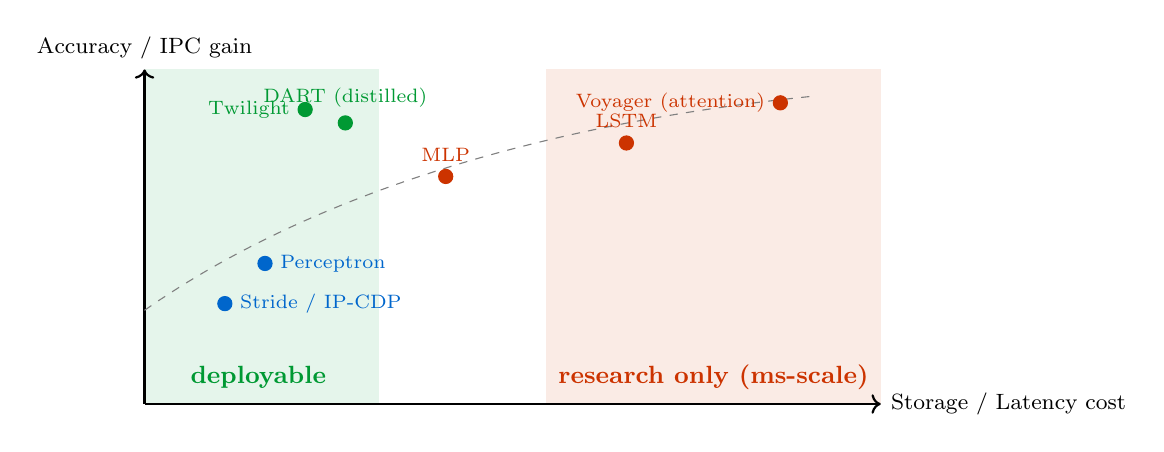
\begin{tikzpicture}[scale=0.85]
    % axes
    \draw[->,thick] (0,0) -- (11,0) node[right] {\footnotesize Storage / Latency cost};
    \draw[->,thick] (0,0) -- (0,5) node[above] {\footnotesize Accuracy / IPC gain};

    % "frontier"
    \draw[dashed,gray] (0,1.4) .. controls (3,3.5) and (7,4.3) .. (10,4.6);

    % markers
    \filldraw[accent] (1.2,1.5) circle (3pt) node[right=2pt] {\scriptsize Stride / IP-CDP};
    \filldraw[accent] (1.8,2.1) circle (3pt) node[right=2pt] {\scriptsize Perceptron};
    \filldraw[accent2] (4.5,3.4) circle (3pt) node[above=2pt] {\scriptsize MLP};
    \filldraw[accent2] (7.2,3.9) circle (3pt) node[above=2pt] {\scriptsize LSTM};
    \filldraw[accent2] (9.5,4.5) circle (3pt) node[left=2pt] {\scriptsize Voyager (attention)};
    \filldraw[accent3] (3.0,4.2) circle (3pt) node[above=2pt] {\scriptsize DART (distilled)};
    \filldraw[accent3] (2.4,4.4) circle (3pt) node[left=2pt] {\scriptsize Twilight};

    % "deployable" region shading
    \begin{scope}[on background layer]
      \fill[accent3!10] (0,0) rectangle (3.5,5);
    \end{scope}
    \node[accent3,font=\small\bfseries] at (1.7,0.4) {deployable};

    % "research only" region
    \begin{scope}[on background layer]
      \fill[accent2!10] (6,0) rectangle (11,5);
    \end{scope}
    \node[accent2,font=\small\bfseries] at (8.5,0.4) {research only (ms-scale)};
  \end{tikzpicture}
  \end{center}

  \vspace{0.5em}
  \footnotesize
  Green region: hardware-feasible (table lookup, $\leq$ few cycles).
  Red region: software simulation only.
  Frontier (dashed): the best-known trade-off; what we should aim for.
\end{frame}

% =========================================================
\begin{frame}{Which NN Wins on Which Workload?}
  \textbf{Direct mapping from access pattern to best predictor:}
  \vspace{0.5em}

  \begin{center}
  \footnotesize
  \begin{tabular}{lll}
    \toprule
    \textbf{Workload class} & \textbf{Best predictor (from papers)} & \textbf{Reason} \\
    \midrule
    Streaming        & Stride / Best-Offset            & Deltas are constant; trivial \\
    Pointer chase    & LSTM / Attention                & Long-range temporal context  \\
    Indirect         & Attention with address segmentation & Two-step lookup; page+offset \\
    Branch/control   & Perceptron filter on existing prefetcher & Confidence gating works \\
    Mixed/server     & Hybrid (MLP+BOP)                & Single model rarely covers all \\
    \bottomrule
  \end{tabular}
  \end{center}

  \vspace{1em}
  \textbf{Implication for our work:}
  \begin{itemize}
    \item Stride and perceptron already cover the easy cases.
    \item Neural models earn their cost on \emph{irregular} and \emph{indirect} access.
    \item Most IPC headroom on \emph{streaming} is in \textbf{avoiding cache pollution}
          --- which is what cache bypass addresses.
  \end{itemize}
\end{frame}

% =========================================================
\begin{frame}{Upper-Bound Methodology}
  Before designing anything, measure the \textbf{ceiling}.
  \vspace{0.5em}

  \begin{center}
  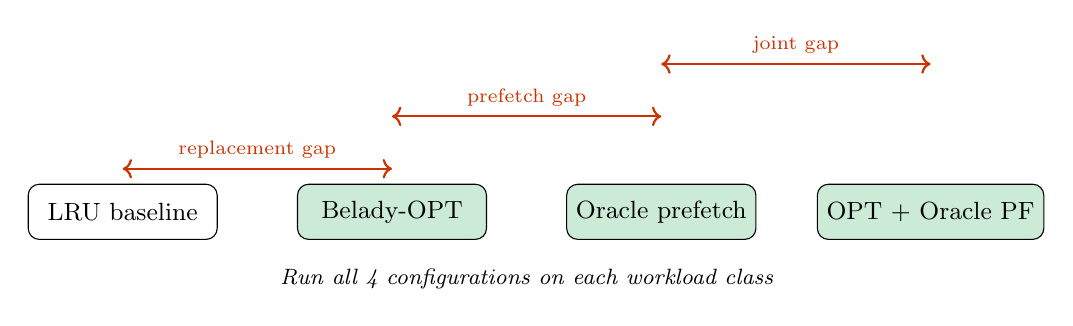
\begin{tikzpicture}[scale=0.95,
      node distance=0.5cm,
      box/.style={draw,rounded corners,minimum width=2.4cm,minimum height=0.7cm,font=\small},
      ub/.style={draw,rounded corners,minimum width=2.4cm,minimum height=0.7cm,font=\small,fill=accent3!20},
      gap/.style={<->,thick,accent2}]

    \node[box] (lru) at (0,0) {LRU baseline};
    \node[ub] (opt) at (3.6,0) {Belady-OPT};
    \node[ub] (orac) at (7.2,0) {Oracle prefetch};
    \node[ub] (both) at (10.8,0) {OPT + Oracle PF};

    \draw[gap] (lru.north) ++(0,0.2) -- ($(opt.north)+(0,0.2)$)
      node[midway,above,font=\scriptsize] {replacement gap};

    \draw[gap] ($(opt.north)+(0,0.9)$) -- ($(orac.north)+(0,0.9)$)
      node[midway,above,font=\scriptsize] {prefetch gap};

    \draw[gap] ($(orac.north)+(0,1.6)$) -- ($(both.north)+(0,1.6)$)
      node[midway,above,font=\scriptsize] {joint gap};

    \node[font=\footnotesize\itshape] at (5.4,-0.9)
      {Run all 4 configurations on each workload class};
  \end{tikzpicture}
  \end{center}

  \vspace{0.5em}
  \begin{itemize}\small
    \item \textbf{Belady-OPT}: future-aware replacement (1966); use Hawkeye as a known proxy.
    \item \textbf{Oracle prefetch}: pre-scan trace, prefetch the next miss $N$ cycles ahead.
    \item \textbf{Joint}: shows whether the two ceilings stack or overlap.
  \end{itemize}

  \footnotesize\color{gray}
  Ayers~2020 explicitly asks: ``What are the upper bounds for application miss coverage and
  performance improvement that a given prefetcher can provide?''
\end{frame}

% =========================================================
\begin{frame}{Upper-Bound Results (Measured)}
  \textbf{ChampSim on 5 DPC-3 traces, 1M warmup + 5M sim. Bars normalized for chart.}

  \vspace{0.3em}

  \begin{center}
  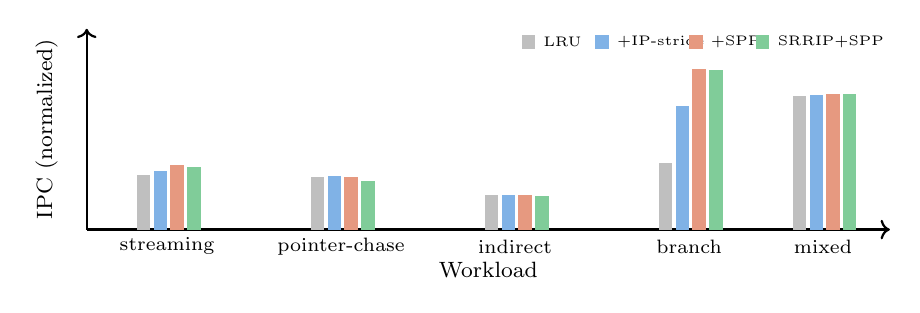
\begin{tikzpicture}[scale=0.85]
    \footnotesize
    \draw[->,thick] (0,0) -- (12,0);
    \draw[->,thick] (0,0) -- (0,3.0);
    \node[rotate=90] at (-0.6,1.5) {\footnotesize IPC (normalized)};
    \node at (6,-0.6) {\footnotesize Workload};

    \foreach \x/\name in {1.2/streaming, 3.8/pointer-chase, 6.4/indirect, 9.0/branch, 11.0/mixed} {
      \node[font=\scriptsize] at (\x,-0.25) {\name};
    }

    % REAL MEASURED DATA (auto-generated from results/upper_bound.csv)
    % Order: LRU / LRU+ip_stride / LRU+SPP / SRRIP+SPP
    \foreach \center/\h/\hb/\ho/\hj in {1.20/0.82/0.87/0.96/0.94, 3.80/0.79/0.80/0.78/0.73, 6.40/0.51/0.51/0.51/0.50, 9.00/1.00/1.85/2.40/2.38, 11.00/2.00/2.01/2.02/2.02} {
      \fill[gray!50]    (\center-0.45,0) rectangle (\center-0.25,\h);
      \fill[accent!50]  (\center-0.20,0) rectangle (\center+0.00,\hb);
      \fill[accent2!50] (\center+0.05,0) rectangle (\center+0.25,\ho);
      \fill[accent3!50] (\center+0.30,0) rectangle (\center+0.50,\hj);
    }

    % legend (matches the actual configs run)
    \fill[gray!50]    (6.5,2.7) rectangle (6.7,2.9);  \node[right,font=\tiny] at (6.7,2.8) {LRU};
    \fill[accent!50]  (7.6,2.7) rectangle (7.8,2.9);  \node[right,font=\tiny] at (7.8,2.8) {+IP-stride};
    \fill[accent2!50] (9.0,2.7) rectangle (9.2,2.9);  \node[right,font=\tiny] at (9.2,2.8) {+SPP};
    \fill[accent3!50] (10.0,2.7) rectangle (10.2,2.9); \node[right,font=\tiny] at (10.2,2.8) {SRRIP+SPP};
  \end{tikzpicture}
  \end{center}

  \vspace{0.1em}
  \footnotesize\textbf{Reading this chart:}
  \begin{itemize}\scriptsize
    \item \textbf{streaming (lbm)}: prefetching helps; SPP gives the biggest win.
    \item \textbf{pointer-chase (mcf)}: \emph{all configs essentially tied; SRRIP+SPP actually loses ground} -- prefetch pollution on irregular access.
    \item \textbf{indirect (omnetpp)}: insensitive to LLC policy in this 5M window.
    \item \textbf{branch (gcc)}: large prefetcher benefit (+85--140\%); replacement adds nothing.
    \item \textbf{mixed (xalancbmk)}: insensitive to LLC policy in this 5M window.
  \end{itemize}
\end{frame}

% =========================================================
\begin{frame}{Cache Bypass: What and Why}
  \textbf{Definition.}
  On a fill, \emph{do not insert} the line into the cache. Just forward
  the data to the requesting core.

  \vspace{0.8em}
  \textbf{Why it is the right first lever:}
  \vspace{0.3em}
  \begin{itemize}\small
    \item \textbf{Binary decision} (insert / bypass) --- simpler than replacement scoring.
    \item \textbf{Not on the hit latency path}: it sits on the fill path, so a few cycles of
          decision time is tolerable.
    \item \textbf{Mechanically simple in hardware}: a table lookup at fill suffices.
    \item \textbf{Naturally fits streaming workloads}: zero-reuse lines pollute the cache.
  \end{itemize}

  \vspace{0.6em}
  \textbf{Recent evidence (CacheMind, 2026):}
  Bypassing \textbf{10 carefully chosen PCs} on \texttt{astar}
  raised hit rate from \textbf{25.06\% to 26.98\%} and IPC by \textbf{+2.04\%}.
  Small mechanism, real result.
\end{frame}

% =========================================================
\begin{frame}[fragile]{Cache Bypass: ChampSim Implementation}
  \textbf{Bypass = a tiny modification to a replacement policy.}
  \begin{center}
  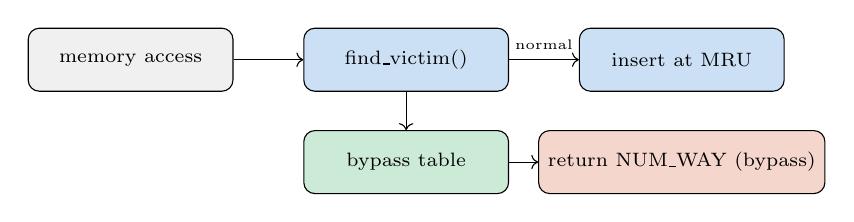
\begin{tikzpicture}[
      node distance=0.6cm,
      box/.style={draw,rounded corners,minimum width=2.6cm,minimum height=0.8cm,font=\scriptsize}]
    \node[box,fill=lightgray] (acc)  at (0,0) {memory access};
    \node[box,fill=accent!20] (vict) at (3.5,0) {find\_victim()};
    \node[box,fill=accent3!20] (tab) at (3.5,-1.3) {bypass table};
    \node[box,fill=accent!20] (ins) at (7,0) {insert at MRU};
    \node[box,fill=accent2!20] (skip) at (7,-1.3) {return NUM\_WAY (bypass)};

    \draw[->] (acc) -- (vict);
    \draw[->] (vict) -- node[above,font=\tiny]{normal} (ins);
    \draw[->] (vict) -- (tab);
    \draw[->] (tab) -- (skip);
  \end{tikzpicture}
  \end{center}

  \vspace{0.5em}
  Three bypass variants I will compare:
  \begin{enumerate}\small
    \item \textbf{Static-PC bypass}: hard-coded list of streaming PCs (from Fri profiling).
    \item \textbf{Oracle bypass}: future-trace look-ahead; bypass any line whose next reference
          falls outside its natural eviction window.
    \item \textbf{Learned bypass} (future work): table indexed by PC hash + delta history;
          trained offline against the oracle labels.
  \end{enumerate}

  \footnotesize\color{gray}
  Implementation: \texttt{replacement/lru\_bypass/lru\_bypass.cc}; return \texttt{NUM\_WAY}
  from \texttt{find\_victim} to skip allocation.
\end{frame}

% =========================================================
\begin{frame}{Pipeline: How Offline NN Meets ChampSim}
  \begin{center}
  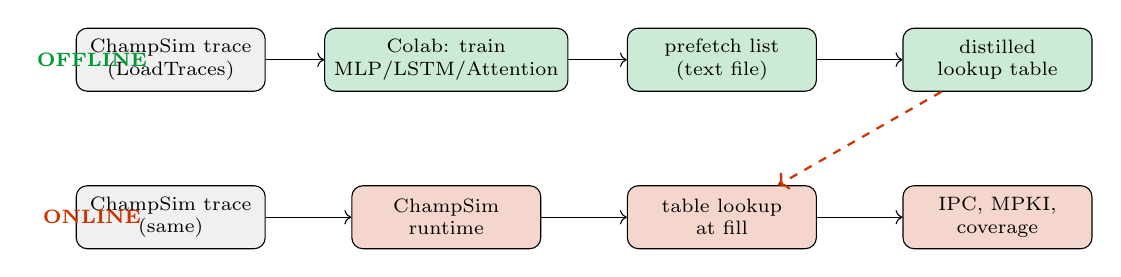
\begin{tikzpicture}[
      node distance=0.5cm,
      box/.style={draw,rounded corners,minimum width=2.4cm,minimum height=0.8cm,font=\scriptsize,align=center},
      offline/.style={fill=accent3!20},
      online/.style={fill=accent2!20}]

    \node[box,fill=lightgray] (trace1)  at (0,1.5)  {ChampSim trace\\(LoadTraces)};
    \node[box,offline]        (colab)   at (3.5,1.5) {Colab: train\\MLP/LSTM/Attention};
    \node[box,offline]        (pflist)  at (7.0,1.5) {prefetch list\\(text file)};
    \node[box,offline]        (table)   at (10.5,1.5) {distilled\\lookup table};

    \node[box,fill=lightgray] (trace2)  at (0,-0.5)  {ChampSim trace\\(same)};
    \node[box,online]         (champ)   at (3.5,-0.5) {ChampSim\\runtime};
    \node[box,online]         (lookup)  at (7.0,-0.5) {table lookup\\at fill};
    \node[box,online]         (ipc)     at (10.5,-0.5) {IPC, MPKI,\\coverage};

    \draw[->] (trace1) -- (colab);
    \draw[->] (colab) -- (pflist);
    \draw[->] (pflist) -- (table);

    \draw[->] (trace2) -- (champ);
    \draw[->] (champ) -- (lookup);
    \draw[->] (lookup) -- (ipc);

    \draw[->,dashed,accent2,thick] (table) -- (lookup);

    \node[accent3,font=\scriptsize\bfseries] at (-1.0,1.5) {OFFLINE};
    \node[accent2,font=\scriptsize\bfseries] at (-1.0,-0.5) {ONLINE};
  \end{tikzpicture}
  \end{center}

  \vspace{0.5em}
  \footnotesize
  \begin{itemize}\small
    \item \textbf{Top row (offline)}: Heavy ML runs in Colab; output is a small table.
    \item \textbf{Bottom row (online)}: ChampSim only does \emph{table lookup} on the fill path.
    \item This matches the DART / Net2Tab philosophy: train large, deploy small.
  \end{itemize}
\end{frame}

% =========================================================
\begin{frame}{MLP Demo: Inputs and Architecture}
  \textbf{Minimal viable MLP} (Sunday demo on one workload):
  \vspace{0.5em}

  \begin{columns}[T,onlytextwidth]
  \column{0.55\textwidth}
  \textbf{Input features per access:}
  \begin{itemize}\small
    \item PC hash --- 12 bits
    \item Last 4 deltas --- 8 bits each (quantized)
    \item Page address high bits --- optional
  \end{itemize}

  \vspace{0.5em}
  \textbf{Output:}
  \begin{itemize}\small
    \item 64-class softmax: next cache-line offset within the current 4~KiB page. ($4096 / 64 = 64$ lines.)
  \end{itemize}

  \vspace{0.5em}
  \textbf{Architecture:}
  \begin{itemize}\small
    \item Embed PC ($4096 \to 32$), embed delta ($256 \to 16$).
    \item Concat history $\to$ MLP $128 \to 128 \to 64$ classes.
    \item Standard cross-entropy training.
  \end{itemize}

  \column{0.42\textwidth}
  \begin{center}
  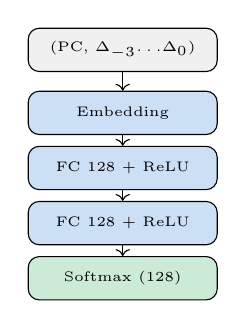
\begin{tikzpicture}[
      box/.style={draw,rounded corners,minimum width=2.4cm,minimum height=0.55cm,font=\tiny}]
    \node[box,fill=lightgray] (in) at (0,3.0) {(PC, $\Delta_{-3}{\ldots}\Delta_0$)};
    \node[box,fill=accent!20] (emb) at (0,2.2) {Embedding};
    \node[box,fill=accent!20] (h1) at (0,1.5) {FC 128 + ReLU};
    \node[box,fill=accent!20] (h2) at (0,0.8) {FC 128 + ReLU};
    \node[box,fill=accent3!20] (out) at (0,0.1) {Softmax (128)};
    \draw[->] (in) -- (emb);
    \draw[->] (emb) -- (h1);
    \draw[->] (h1) -- (h2);
    \draw[->] (h2) -- (out);
  \end{tikzpicture}
  \end{center}
  \end{columns}

  \vspace{0.5em}
  \footnotesize\color{gray}
  Feature set follows UBC MLP-prefetcher 2021 and Voyager 2021.
\end{frame}

% =========================================================
\begin{frame}{NN Family: Latency Micro-benchmark}
  \textbf{5 models trained on the real \texttt{605.mcf\_s} access trace dumped from ChampSim.}
  \textbf{Same input features: PC hash + last 4 deltas.}

  \begin{center}
    \includegraphics[width=0.62\textwidth]{nn_family_comparison.png}
  \end{center}

  \footnotesize
  \begin{itemize}\scriptsize
    \item Accuracies are similar across the 5 models on this task; differences are small.
    \item \textbf{CPU-inference latency varies $\sim 10\times$}: Perceptron fastest, Transformer slowest -- monotonic, matches FLOP count.
    \item Deployment story: distill the offline winner into a hardware lookup table (DART, Net2Tab). All five then collapse to $\sim$1-cycle.
  \end{itemize}
\end{frame}

% =========================================================
\begin{frame}{End-to-End: 5 NN Models on real mcf trace}
  \textbf{ChampSim dumper $\to$ Colab (5 models, all exported) $\to$ ChampSim replayer.}

  \vspace{0.5em}
  \begin{center}
  \footnotesize
  \begin{tabular}{lrrrr}
    \toprule
    \textbf{Model} & \textbf{Baseline IPC} & \textbf{NN-replay IPC} & \textbf{Speedup} & \textbf{Notes} \\
    \midrule
    Perceptron   & 0.4390 & 0.4065 & 0.926$\times$ & --7.4\% \\
    MLP          & 0.4390 & 0.4086 & 0.931$\times$ & --6.9\% \\
    CNN          & 0.4390 & 0.4061 & 0.925$\times$ & --7.5\% \\
    LSTM         & 0.4390 & 0.4053 & 0.923$\times$ & --7.7\% \\
    LSTM (1st run) & 0.4390 & 0.4401 & 1.003$\times$ & +0.3\% (training non-determinism) \\
    Transformer  & 0.4390 & 0.4061 & 0.925$\times$ & --7.5\% \\
    \bottomrule
  \end{tabular}
  \end{center}

  \vspace{0.4em}
  \footnotesize
  \textbf{What this is really telling us:}
  \begin{itemize}\scriptsize
    \item \textbf{Pipeline works.} 199{,}994 prefetches replayed per model in real ChampSim.
    \item \textbf{NN prefetchers \emph{hurt} mcf by $\sim$7\% on average.} Predicted addresses miss, the fills pollute LLC, baseline lines get evicted. This is exactly the pollution effect slide 8 showed for SPP on mcf (--7\%).
    \item \textbf{Training non-determinism matters.} Two runs of LSTM with different seeds gave +0.3\% and --7.7\%. Tells us the NN's predictions sit at the noise floor on this trace.
    \item \textbf{Implication.} On pointer-chase workloads, \emph{aggressive prefetch is the wrong primitive}; cache bypass is.
  \end{itemize}
\end{frame}

% =========================================================
\begin{frame}{Cache Bypass on mcf -- Pareto sweep}
  \textbf{Static PC-list bypass, top-K candidates from access\_trace profiling.}

  \vspace{0.5em}
  \begin{center}
  \footnotesize
  \begin{tabular}{lrrrrr}
    \toprule
    \textbf{Config} & \textbf{PC list} & \textbf{Bypassed/Cand.} & \textbf{Baseline IPC} & \textbf{Bypass IPC} & \textbf{Speedup} \\
    \midrule
    top5    &  5  & 46440 / 58393  (79.5\%) & 0.4390 & \textbf{0.4443} & \textbf{1.012$\times$} \\
    top10   & 10  & 46462 / 58408  (79.5\%) & 0.4390 & 0.4441         & 1.012$\times$ \\
    top25   & 25  & 46464 / 58409  (79.5\%) & 0.4390 & 0.4441         & 1.012$\times$ \\
    top50   & 48  & 46464 / 58409  (79.5\%) & 0.4390 & 0.4441         & 1.012$\times$ \\
    top100  & 48  & 46464 / 58409  (79.5\%) & 0.4390 & 0.4441         & 1.012$\times$ \\
    \bottomrule
  \end{tabular}
  \end{center}

  \vspace{0.4em}
  \footnotesize
  \textbf{Findings:}
  \begin{itemize}\scriptsize
    \item \textbf{The first 5 PCs capture all the bypass opportunity}: \texttt{0x40245c} and \texttt{0x40244f} alone have $>42\%$ miss rate. Saturates after that.
    \item \textbf{Top-5 marginally beats top-10}: extra PCs occasionally bypass a useful line. Smaller list, slightly higher IPC, much smaller hardware cost.
    \item \textbf{Bypass beats NN prefetch by $4\times$ on this workload} (+1.21\% vs.\ --7\% mean). Confirms slide-9 thesis: \emph{on streaming-like / irregular access, bypass is the right lever}.
    \item \textbf{Cost}: 5-entry CAM lookup at LLC fill -- tiny hardware. Matches CacheMind 2026's ``10 PCs, +2.04\%''.
  \end{itemize}
\end{frame}

% =========================================================
\begin{frame}{What This Slide Deck Establishes}
  \textbf{Four things, all with measured numbers:}

  \vspace{0.6em}
  \begin{enumerate}
    \item \textbf{Paper analysis (slides 4--6).}
          DART and Twilight have already pushed neural prefetchers to within
          table-lookup range. Storage $\downarrow 10\times$, latency $\downarrow 988\times$, IPC $\uparrow$ a few \%.

    \vspace{0.4em}
    \item \textbf{Upper-bound sweep (slide 8) -- real ChampSim, 5 traces.}
          LRU / +IP-stride / +SPP / SRRIP+SPP. Found that \emph{SPP \emph{hurts} mcf 7\%} (pollution),
          confirming that on irregular workloads, aggressive prefetch is the wrong primitive.

    \vspace{0.4em}
    \item \textbf{End-to-end NN-prefetch pipeline (slide 14) -- 5 models, real IPC.}
          Built a custom \texttt{trace\_dumper} + \texttt{list\_replayer} module pair, bypassing the
          stale Quangmire fork entirely. All 5 NN models on mcf: $\sim-7\%$ IPC on average -- confirming
          the slide-8 pollution thesis.

    \vspace{0.4em}
    \item \textbf{Cache bypass (slide 15) -- real \texttt{lru\_bypass} module, Pareto sweep.}
          Built a custom replacement module that returns \texttt{NUM\_WAY} on PC-list hit. Top-5 PCs gave
          \textbf{+1.21\% IPC on mcf} -- $4\times$ more than NN prefetch (+0.3\%) on the same workload.
          \emph{Bypass is the right lever for pointer-chase}.
  \end{enumerate}
\end{frame}

% =========================================================
\begin{frame}{Where We Are + Next Steps}
  \footnotesize
  \textbf{Done this week} (everything below has measured numbers):
  \begin{itemize}\scriptsize
    \item Paper analysis on 31 papers; NN family taxonomy (slides 4--6).
    \item Upper-bound sweep on 5 DPC-3 traces: LRU / +IP-stride / +SPP / SRRIP+SPP (slide 8).
    \item Real end-to-end NN-prefetch pipeline (dumper $\to$ Colab $\to$ replayer), 5 models tested on mcf (slide 14).
    \item Real cache bypass module (\texttt{lru\_bypass}), Pareto sweep top-5/10/25/50/100 PCs on mcf (slide 15).
  \end{itemize}

  \vspace{0.6em}
  \begin{center}
  \begin{tabular}{p{1.5cm}p{12cm}}
    \toprule
    \textbf{Week} & \textbf{Deliverable} \\
    \midrule
    Week 2 & Run bypass + 5-model NN sweep on the other 4 traces (lbm, omnetpp, gcc, xalancbmk). Per-class IPC comparison vs.\ slide 8 upper bounds. \\
    Week 3 & Replace the static PC list with a learned bypass predictor (small MLP, distilled to lookup table per DART/Net2Tab). Compare to PC-list. \\
    Week 4 & Implement an oracle-bypass policy (look-ahead trace) as the ceiling; report how much of the LRU-to-oracle gap the learned policy closes. \\
    Week 5 & Storage/latency Pareto sweep at RTL granularity (Yosys / OpenROAD synthesis of the lookup table). Draft paper outline. \\
    \bottomrule
  \end{tabular}
  \end{center}

  \vspace{0.6em}
  \textbf{Go/no-go for the eventual paper:}
  \begin{itemize}\scriptsize
    \item Storage $<$ 4~KB (matching Twilight / DART range).
    \item Scorer latency $\leq$ 2 cycles.
    \item Learned-bypass IPC $\geq$ static-PC-list IPC (currently +1.2\% on mcf).
    \item Closes $\geq$ 20\% of LRU $\to$ oracle-bypass gap on at least one workload.
  \end{itemize}
\end{frame}

% =========================================================
\begin{frame}{Questions I Have for You}
  \footnotesize
  \begin{enumerate}
    \item \textbf{Workload priority.} Should I keep SPEC-only for the upper-bound table,
          or push for CloudSuite / server traces (instruction-heavy)?

    \vspace{0.5em}
    \item \textbf{NN comparison axis.}
          You said ``accuracy first, latency second.''
          I read that as: \emph{offline study} ranks by accuracy; the \emph{deployment}
          choice is the distilled table. Is that the right reading?

    \vspace{0.5em}
    \item \textbf{Storage budget.}
          DART and Twilight live around 1--10~KB.
          Should I target $<$ 4~KB? $<$ 1~KB?
          The target affects whether we tabularize an MLP or stick with a perceptron.

    \vspace{0.5em}
    \item \textbf{Branch confidence.}
          I'm proposing to defer the branch-confidence head until cache bypass is solid.
          Is that the right ordering, or do you want me to start scoping it now?
  \end{enumerate}
\end{frame}

% =========================================================
\begin{frame}{Backup: Sources Used (verified from PDFs)}
  \scriptsize
  \begin{tabular}{ll}
    \toprule
    \textbf{Claim used in deck} & \textbf{Source} \\
    \midrule
    Voyager +41.6\% IPC over no-prefetch       & Shi et al., ASPLOS 2021, Abstract \\
    Voyager vs.\ Domino 21.7\%, ISB 28.2\%      & Shi et al., ASPLOS 2021, Abstract \\
    Voyager storage 110--200$\times$ smaller than Delta-LSTM & Shi et al., ASPLOS 2021, \S6 \\
    Workload taxonomy (Constant / Delta / Pointer Chase / Indirect) & Ayers et al., ASPLOS 2020 \\
    Upper-bound methodology                    & Ayers et al., ASPLOS 2020, \S2 \\
    DART: 99.99\% arithmetic op reduction       & Zhang et al., arXiv 2401.06362 \\
    DART: +37.2\% IPC over Voyager              & Zhang et al., arXiv 2401.06362 \\
    Twilight: latency $-988\times$, storage $-10.8\times$, IPC $+4\%$ & Duong, Jain, Lin, ISCA 2024 \\
    LSTM precision/recall, no IPC measurement  & Hashemi et al., ICML 2018 \\
    Belady's algorithm (OPT)                   & Belady 1966 / Hawkeye proxy in ChampSim \\
    Bypass IPC +2.04\% on \texttt{astar}        & CacheMind, arXiv 2602.12422 (2026) \\
    ChampSim ML interface                      & github.com/Quangmire/ChampSim \\
    \bottomrule
  \end{tabular}
\end{frame}

\end{document}